\subsection{Preprocesamiento De Los Datos} 
Con el objetivo de darle mayor estabilidad matemática a los datos y quitar el ruido que puedan tener, realizamos un preprocesamiento de los mismos. El mismo consistió en quitar los outliers dentro del set de datos y luego normalizarlos con media $0$ y varianza $1$.

\subsection{Implementación Del algoritmo} 

El algoritmo implementado consistió en una red neuronal profunda con retropropagación del error. Este, descripto de manera informal consiste para cada instancia del problema, calcular la salida, compararla con la salida esperada y retropropagar el error, con el objetivo modificar las matrices de pesos e ir minimizando las diferencias entre la salida esperada y la obtenida.

Escribiendo de manera formal el algoritmo, sea $L$ la cantidad de capas, $S$ la cantidad de nodos de cada capa, $y_i$ las distintas capas de $1$ a $L$ y $f_i(x)$ la función de activación de la capa $i$:

\begin{algorithm}[h!]
\begin{algorithmic}[1]\parskip=1mm
 \caption{Activación(x)}
 \STATE{$y_1 = x$}
 \STATE{$for j \in [2..L]$}
 \STATE{\quad $y_j \leftarrow f_j(y_{j-1}.W_j)$}
 \STATE{return $y_L$}
\end{algorithmic}
\end{algorithm}

En este pseudocódigo se toma la entrada y se fowardea por todas las capas hasta llegar a la ultima. La capa $y_L$ será el resultado de la red.

\pagebreak

\begin{algorithm}[h!]
\begin{algorithmic}[1]\parskip=1mm
 \caption{Corrección($z$)}
 \STATE{$E = (z-y_L)$}
 \STATE{$e = \|E\|^2$}
 \STATE{for $j \in [2..L]$}
 \STATE{\quad $D \leftarrow E.f'(y_j-1.W_j)$}
 \STATE{\quad $\bigtriangleup W_j \leftarrow dw_j + \Delta (D.Y_{j-1})$}
 \STATE{\quad $E \leftarrow D.W^T_j$}
 \STATE{ret $e$}
\end{algorithmic}
\end{algorithm}

En la etapa de corrección se toma el resultado de la red $y_L$, se compara con el resultado esperado $z$ y se retropropaga el error corrigiendo en cada capa.

\begin{algorithm}[h!]
\begin{algorithmic}[1]\parskip=1mm
 \caption{Adaptación($z$)}
 \STATE{for $h \in [1..L]$}
 \STATE{\quad $W_j \leftarrow W_j + \bigtriangleup W_j$}
 \STATE{\quad $\bigtriangleup W_j \leftarrow 0$}
\end{algorithmic}
\end{algorithm}

En esta etapa se actualizarán las matrices $W$ con los nuevos pesos una vez que haya terminado la fase de corrección.

El esquema general del algoritmo será el siguiente:

\begin{algorithm}[h!]
\begin{algorithmic}[1]\parskip=1mm
 \caption{Entrenamiento($z$)}
 \STATE{$e \rightarrow 0$}
 \STATE{for $h \in [1..P]$}
 \STATE{\quad $z_h \leftarrow Activacion(x_h)$}
 \STATE{\quad $e \leftarrow Correcion(z_h)$}
 \STATE{\quad adaptación()}
\end{algorithmic}
\end{algorithm}

El sistema implementado se dice ser $online$ ya que los pesos de las matrices son ajustados luego de retropropagar el error de cada instancia en vez de hacerlo al final de la época.

A fin de tener una medida de como va "aprendiendo" la red neuronal, luego de presentarle a la red todas las instancias una vez, calculamos la norma de todos los $e$ obtenidos. Consideraremos esta nuestra "norma del error" y la utilizaremos como una métrica adecuada para saber cuan buenos resultados devuelve nuestra red.

%habria que poner pseudocodigo o algo mas lindo acá

%falta explicar un poco mejor las funciones de activacion que usamos, etc

Como optimización adicional se agrego un termino de momentum. La idea tras esto consiste en darle a cada peso de la matriz una "inercia" que le permita continuar avanzando en la dirección en la que avanzó en la iteración anterior. El objetivo consiste en disminuir las oscilaciones con cada pequeño cambio en la matriz.

Para la implementación del código, utilizamos Python y la librería matemática numpy que nos facilitó la utilización de operaciones matriciales. 

\subsection{Experimentación sobre datos de Diagnostico de Cáncer}

\subsubsection{Convergencia del algoritmo} 

%decir que usamos logistica porque es una clasificacion idem l.12

Para este problema utilizaremos una neurona en la última capa con función de activación logística. Para ser consistentes con esto, las salidas esperadas adoptarán los valores $1$ si resulto ser cáncer maligno, y $0$ si resulto ser benigno. La experimentación consistirá en buscar los parámetros óptimos que nos den la mayor tasa de aciertos para nuestro data set.

Como primera instancia comprobaremos que la red converge efectivamente a la solución esperada. Para eso tomamos un learning rate de $0.01$, $7$ neuronas en la capa oculta y con $1300$ épocas graficamos la norma del error cada $1000$ iteraciones:

\begin{figure}[h!]
  \centering
    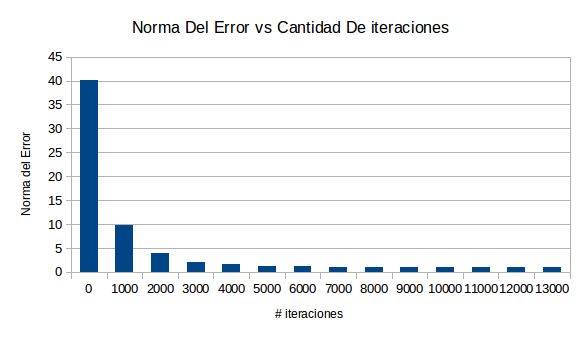
\includegraphics[scale=0.4]{ej1/convergencia.png}
\end{figure}

El gráfico muestra que, efectivamente, nuestro algoritmo minimiza la diferencia entre las soluciones obtenidas y las deseadas, minimizando así también la norma del error.

En las secciones subsiguientes, realizaremos diferentes experimentaciones sobre los hiperparametros del algoritmo para intentar aproximar a la solución ideal.

\subsubsection{Performance Vs Learning Rate} 

%Capaz va mas arriba?
Para evitar el sobreajuste todas las experimentaciones desde este punto se realizarán con la siguiente metodología. Se dividirá el set de datos de entrenamiento provisto por la cátedra en dos sets de datos distintos. Uno se utilizará para entrenar la red, mientras que en el otro se medirán que tan buenos fueron los resultados obtenidos. Con esto se espera reducir el overfittning que la red pueda generar y comprobar de manera mas acertada que tan buenos resultados dará la red sobre datos reales del problema.

Además, para visualizar los resultados mas claramente utilizaremos una matriz de confusión, que nos permitirá discernir entre falsos positivos (fp), falsos negativos(fn) y instancias clasificadas correctamente (tp y tn).

En esta sección buscaremos sacar conclusiones observando que sucede con los resultados obtenidos al variar el learning rate. Para ello, dejamos constantes las cantidad de épocas de entrenamiento en $10000$ y para una capa oculta con $7$ neuronas, variamos el learning desde $0.01$ hasta $0.2$ aumentando de a $0.01$

\begin{figure}[h!]
\centering
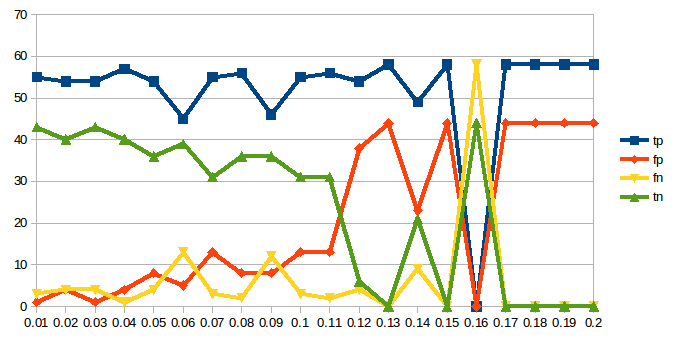
\includegraphics[scale=0.4]{ej1/test_learning_rate.png}
\end{figure}

El gráfico muestra varios resultados interesantes. En el rango $[0.01,0.11]$ puede verse que la red arroja buenos resultados, obteniendo en general un $90\%$ de clasificaciones correctas. Pasado ese rango puede verse como los falsos positivos y los falsos negativos sufren un incremento muy significativo, llegando al final a casi un $50\%$ de clasificaciones incorrectas. Consideramos que para estos casos la red neuronal divergió, posiblemente debido a que multiplicar el gradiente por un valor muy grande lleva a "pasarnos" del mínimo y por lo tanto reduciendo la precisión del algoritmo.

A partir de esta experimentación, para los siguientes experimentos decidimos tomar un learning rate igual a $0.02$. Consideramos que uno mayor puede producir que el algoritmo diverja, mientras que uno mas pequeño hará que tarde demasiado en alcanzar la solución final.

\subsubsection{Performance Vs Cantidad De Neuronas} 

El siguiente experimento a realizar es ver el comportamiento de los resultados dependiendo de la cantidad de neuronas en la capa oculta de la red. Para testear esto mantenemos la cantidad de iteraciones y el learning rate fijos en $1000$ y $0.02$ respectivamente y variamos la cantidad de neuronas desde $1$ a $20$.

Los resultados obtenidos se grafican en el siguiente gráfico:

\begin{figure}[h!]
\centering
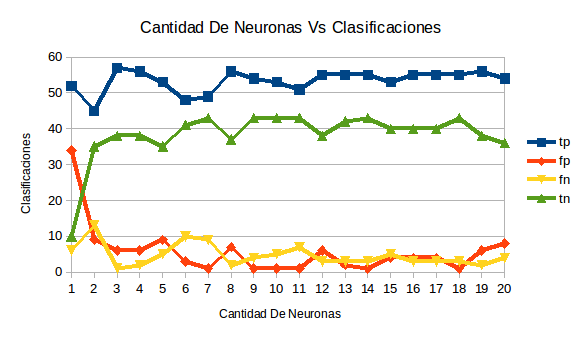
\includegraphics[scale=0.4]{ej1/test_neuronas.png}
\end{figure}

Como puede observarse, una cantidad de neuronas muy pequeña reduce considerablemente la calidad de los resultados. Esto puede deberse a que, según simon O. Haykin la capa oculta funciona como un detector de características. A medida que la red va aprendiendo las neuronas de la capa oculta comienzan a descubrir las características sobresalientes en los datos de entrenamiento, pudiendo hacer mas fácil la separación de las dos clases del problema. Por este motivo consideramos que, al tener pocas neuronas en la capa oculta no es posible para la red encontrar suficientes características y por lo tanto los resultados empeoran.

En este caso decidimos utilizar una cantidad de neuronas igual a $3$. Si bien dijimos que una mayor cantidad de neuronas aumenta la cantidad de características "descubiertas", puede suceder que para un numero excesivo de neuronas estas características empiecen a repetirse o que la red simplemente memorice las características de la entrada, resultando en un mayor overfitting de la red.

\subsubsection{Performance Vs Cantidad De iteraciones} 

Como siguiente paso buscaremos analizar el comportamiento de la red para distintas cantidades de iteraciones, viendo si existe algún cambio significativo en este sentido. Para ello dejamos fijo el learning rate fijo en $0.02$, la cantidad de neuronas en $3$ y variamos la cantidad de iteraciones.

\begin{figure}[h!]
  \centering
    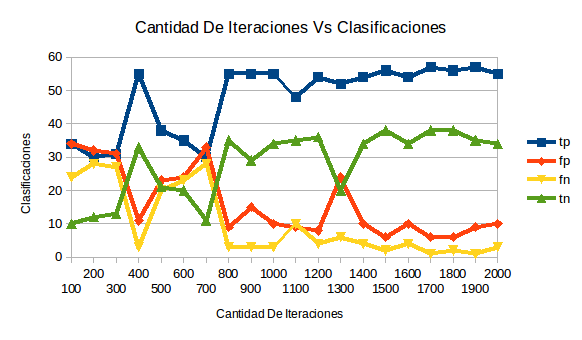
\includegraphics[scale=0.4]{ej1/iteraciones.png}
\end{figure}

Para una cantidad menor a $600$ iteraciones puede observarse que la red neuronal tiene una performance mala obteniendo un porcentaje de falsos negativos y falsos positivos cercano al $50\%$. Ya con $700$ iteraciones en adelante la performance del algoritmo mejora drásticamente, rondando el porcentaje de falsos negativos y falsos positivos al rededor de $10 \%$ y $20\%$. Para $2000$ y $2100$ iteraciones obtenemos un $7\%$  de falsos negativos.

Decidimos utilizar una cantidad de iteraciónes igual a $900$. El motivo de esta elección reside en lo antes expuesto, una cantidad menor produce que el algoritmo todavía no converja a la solución ideal, mientras que una cantidad mayor, si bien parece aumentar la precisión de la solución, también podría deberse al overfitting de los datos.

\subsection{Eficiencia energética} 

Este problema presenta ciertas diferencias con respecto al anterior. En particular en este caso querremos hacer una regresión lineal sobre los datos. Por lo tanto, elegimos una función de activación lineal en la ultima capa. Además para cada conjunto de atributos se deberán devolver dos resultados diferentes, por lo que la ultima capa tendrá dos neuronas de salida.

\subsubsection{Convergencia del algoritmo}

De igual manera que para el caso del cáncer de mama, lo primero que querremos determinar es que el algoritmo converge a la solución deseada. Por lo que nuevamente tomamos un learning rate de $0.01$, $30$ neuronas en la capa oculta y con $100000$ épocas graficamos la norma del error cada $1000$ iteraciones:


\begin{figure}[h!]
  \centering
    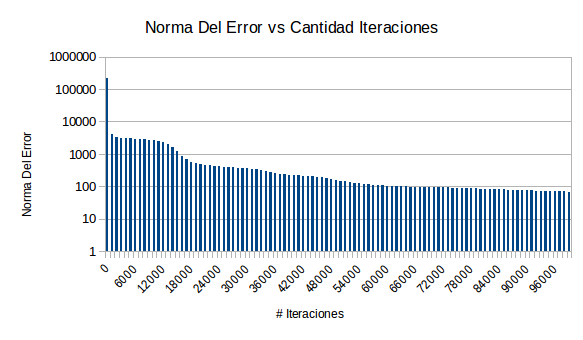
\includegraphics[scale=0.4]{ej2/convergencia.png}
\end{figure}

A simple vista se puede notar que en este caso el algoritmo converge de manera mucho mas lenta (notar que el gráfico se encuentra en escala logarítmica). Nuestro siguiente objetivo será ajustar los parámetros de manera adecuada para intentar que la solución devuelta por el algoritmo sea lo mas aproximada a la solución exacta.

\subsubsection{Performance Vs Learning Rate}

En esta sección esperamos determinar un learning rate adecuado para nuestro algoritmo. A priori pareciera que $0.01$ resulta muy bajo para este caso, resultando en una convergencia muy lenta. Para este experimento dejamos la cantidad de épocas fija en $10000$, la cantidad de neuronas de la capa oculta en $30$ y variamos el learning rate desde $0.01$ a $0.2$ con un step de $0.01$. Los resultados obtenidos fueron:

\begin{figure}[h!]
  \centering
    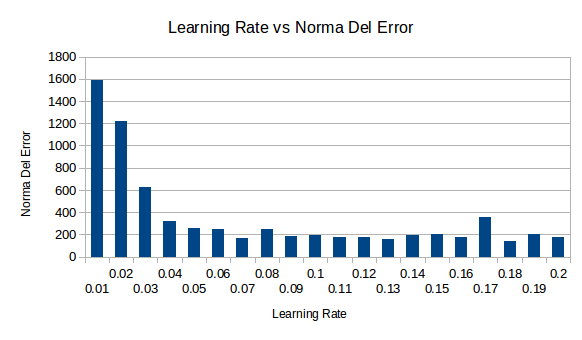
\includegraphics[scale=0.4]{ej2/test_learning_rate.png}
\end{figure}

Como puede verse, en este caso un learning rate mayor aumenta considerablemente la convergencia del algoritmo.

Por este motivo, elegimos como nuestro learning rate óptimo el de $0.05$. Consideramos que un learning rate excesivo, si bien puede reducir la norma del error a niveles mayores, puede producir que el algoritmo no generalice las soluciones y simplemente memorice las instancias de entrenamiento.

\subsubsection{Cantidad De neuronas Vs Performance}

Al igual que en el caso del cáncer, queremos ver como afecta la cantidad de neuronas a los resultados. Para ello nos basamos en el experimento anterior para obtener un learning rate que consideramos aceptable, dejamos la cantidad de iteraciones en $10000$ y variamos la cantidad de neuronas desde $1$ a $20$.

\begin{figure}[h!]
  \centering
    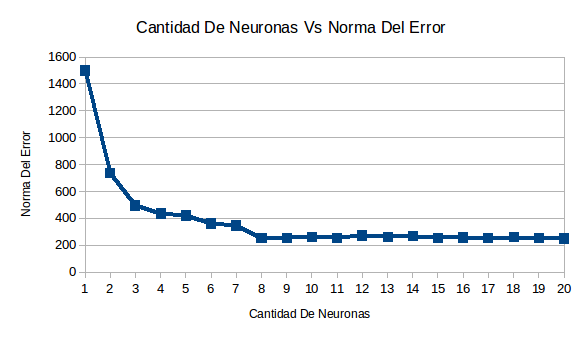
\includegraphics[scale=0.4]{ej2/test_neuronas.png}
\end{figure}

En el gráfico puede observarse que para una cantidad muy pequeña de neuronas, los resultados resultan mucho peores. Aumentando la cantidad de neuronas a $3$ ya la norma del error mejora sustancialmente, mientras que para una cantidad mayor de neuronas el algoritmo parece alcanzar una meseta.

Por este motivo Consideramos que para este caso la cantidad óptima de neuronas es $8$ y trabajaremos con este numero de neuronas en las siguientes experimentaciónes.

%hablar sobre el overfitting si usamos parametros mayores o algo asi.

\subsubsection{Épocas Vs Performance}

Como experimento final para esta sección buscaremos encontrar cual es la cantidad óptima de iteraciones para este algoritmo. Para ello utilizaremos los parámetros que consideramos mejores en la experimentación anterior (cantidad de neuronas $= 8$ y learning rate $= 0.02$) y variamos la cantidad de épocas desde $2000$ hasta $21000$:

\begin{figure}[h!]
  \centering
    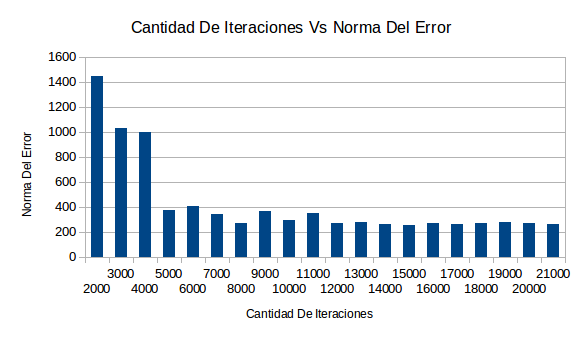
\includegraphics[scale=0.4]{ej2/test_iteraciones.png}
\end{figure}

Para $2000$ a $4000$ épocas, es correcto asumir que el algoritmo todavía no había convergido a una solución, encontrándose la norma del error en el orden de los $1000$. Desde las $5000$ iteraciones en adelante puede verse que el error cae repentinamente y se estabiliza en aproximadamente $200$.  

Por este motivo Consideramos tomar para este caso una cantidad de épocas igual a $7000$.

%TODO: concluciones de cada apartado
